\section{Objets d'exemples}
\subsection{Images et tableaux}
\subsubsection{Images}
\myparagraph{Image centrée}

\begin{figure}[h] 
    \caption{Photo d'un micro poussièreux - Gaël Germain - 08/09/24}
    \centering
    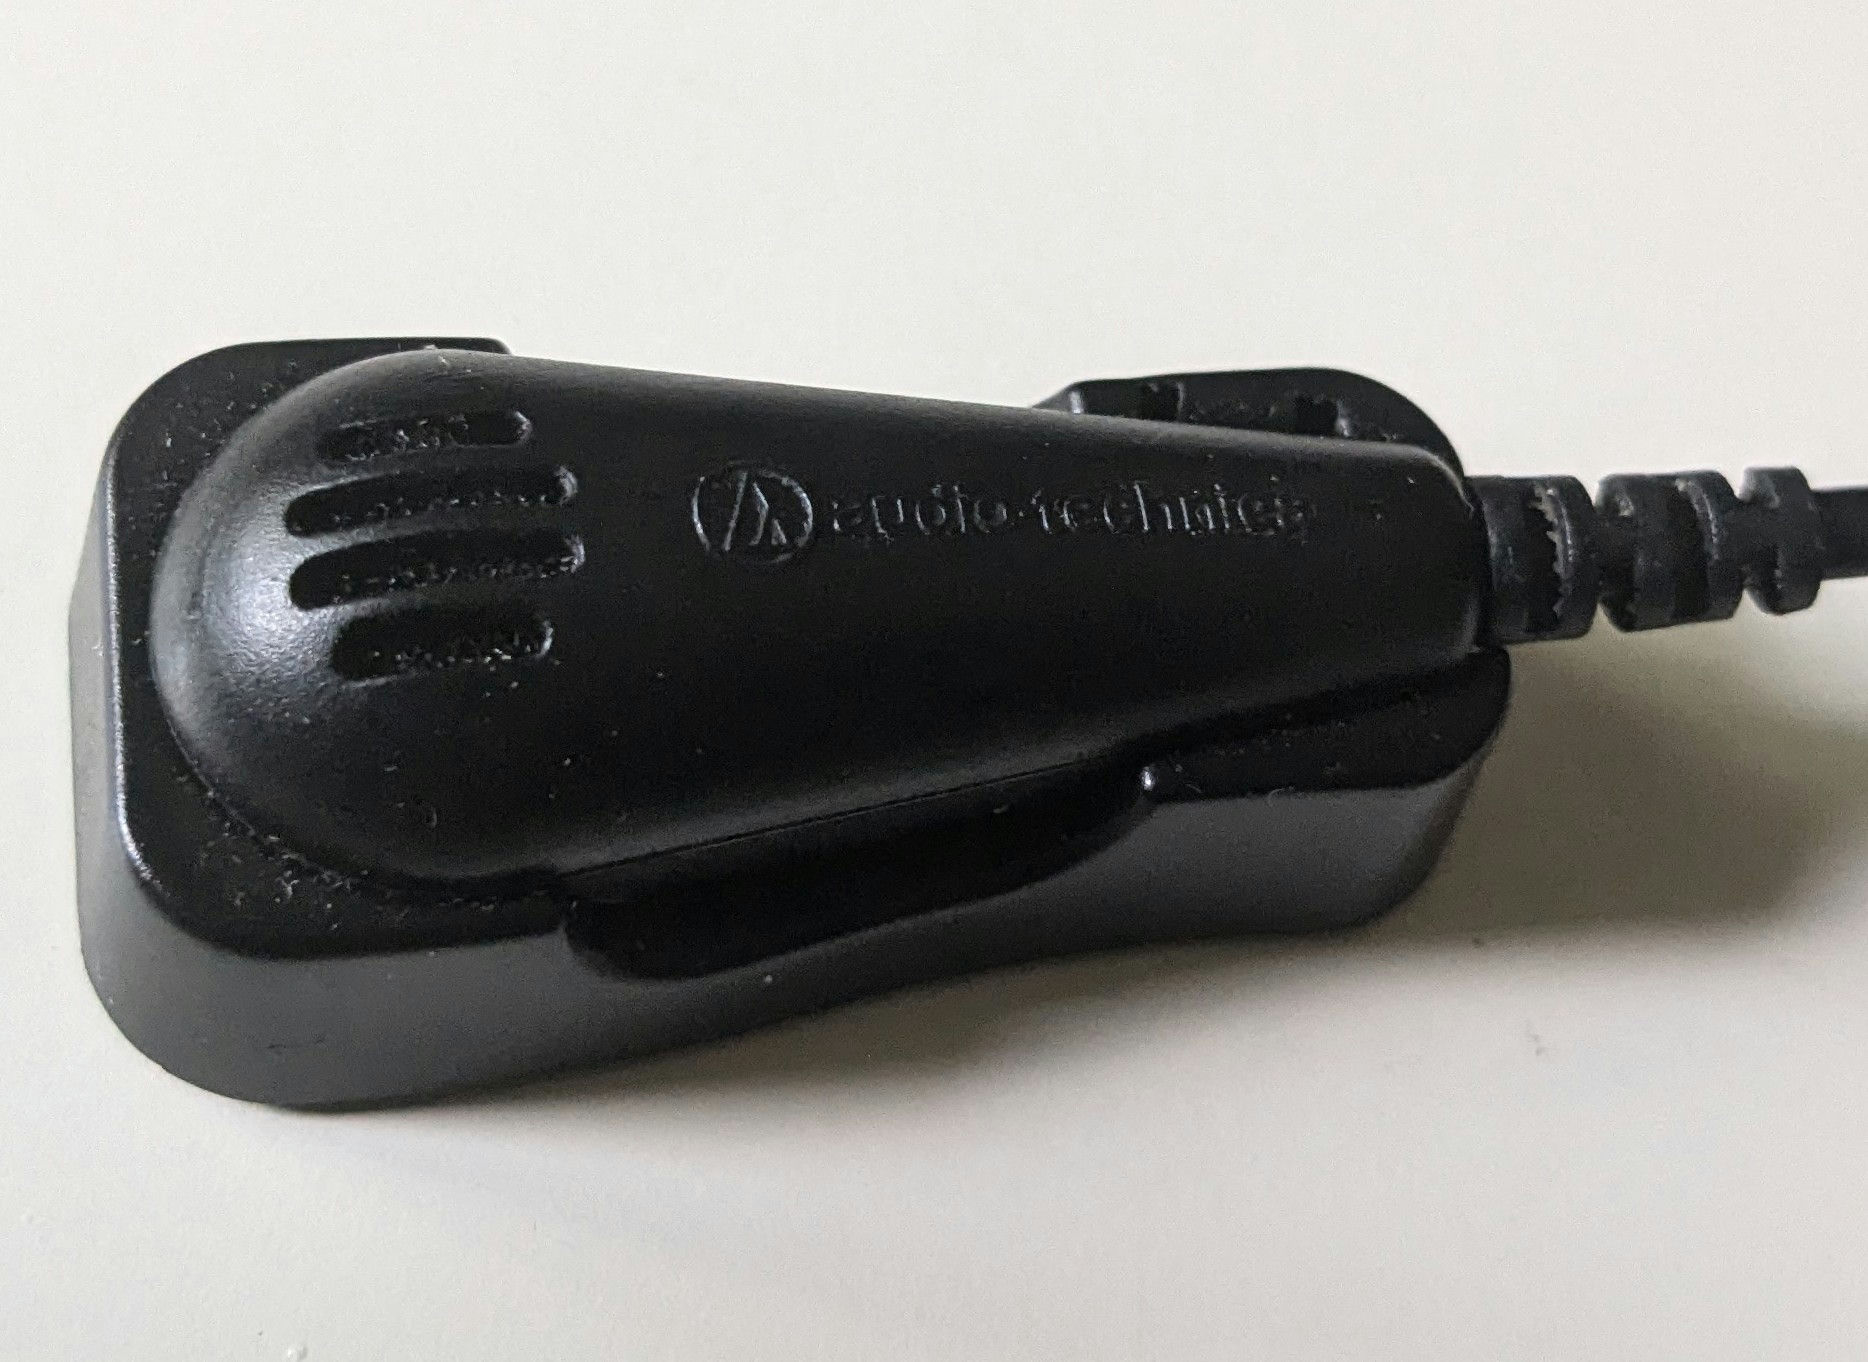
\includegraphics[width=0.7\textwidth]{images/micro_poussiereux.jpg}
\end{figure}

\myparagraph{Image entourée de texte}

\begin{wrapfigure}{r}{0.35\textwidth}
    %\vspace{-1cm}
    \centering
    \caption{Photo d'un micro poussièreux - Gaël Germain - 08/09/24}
    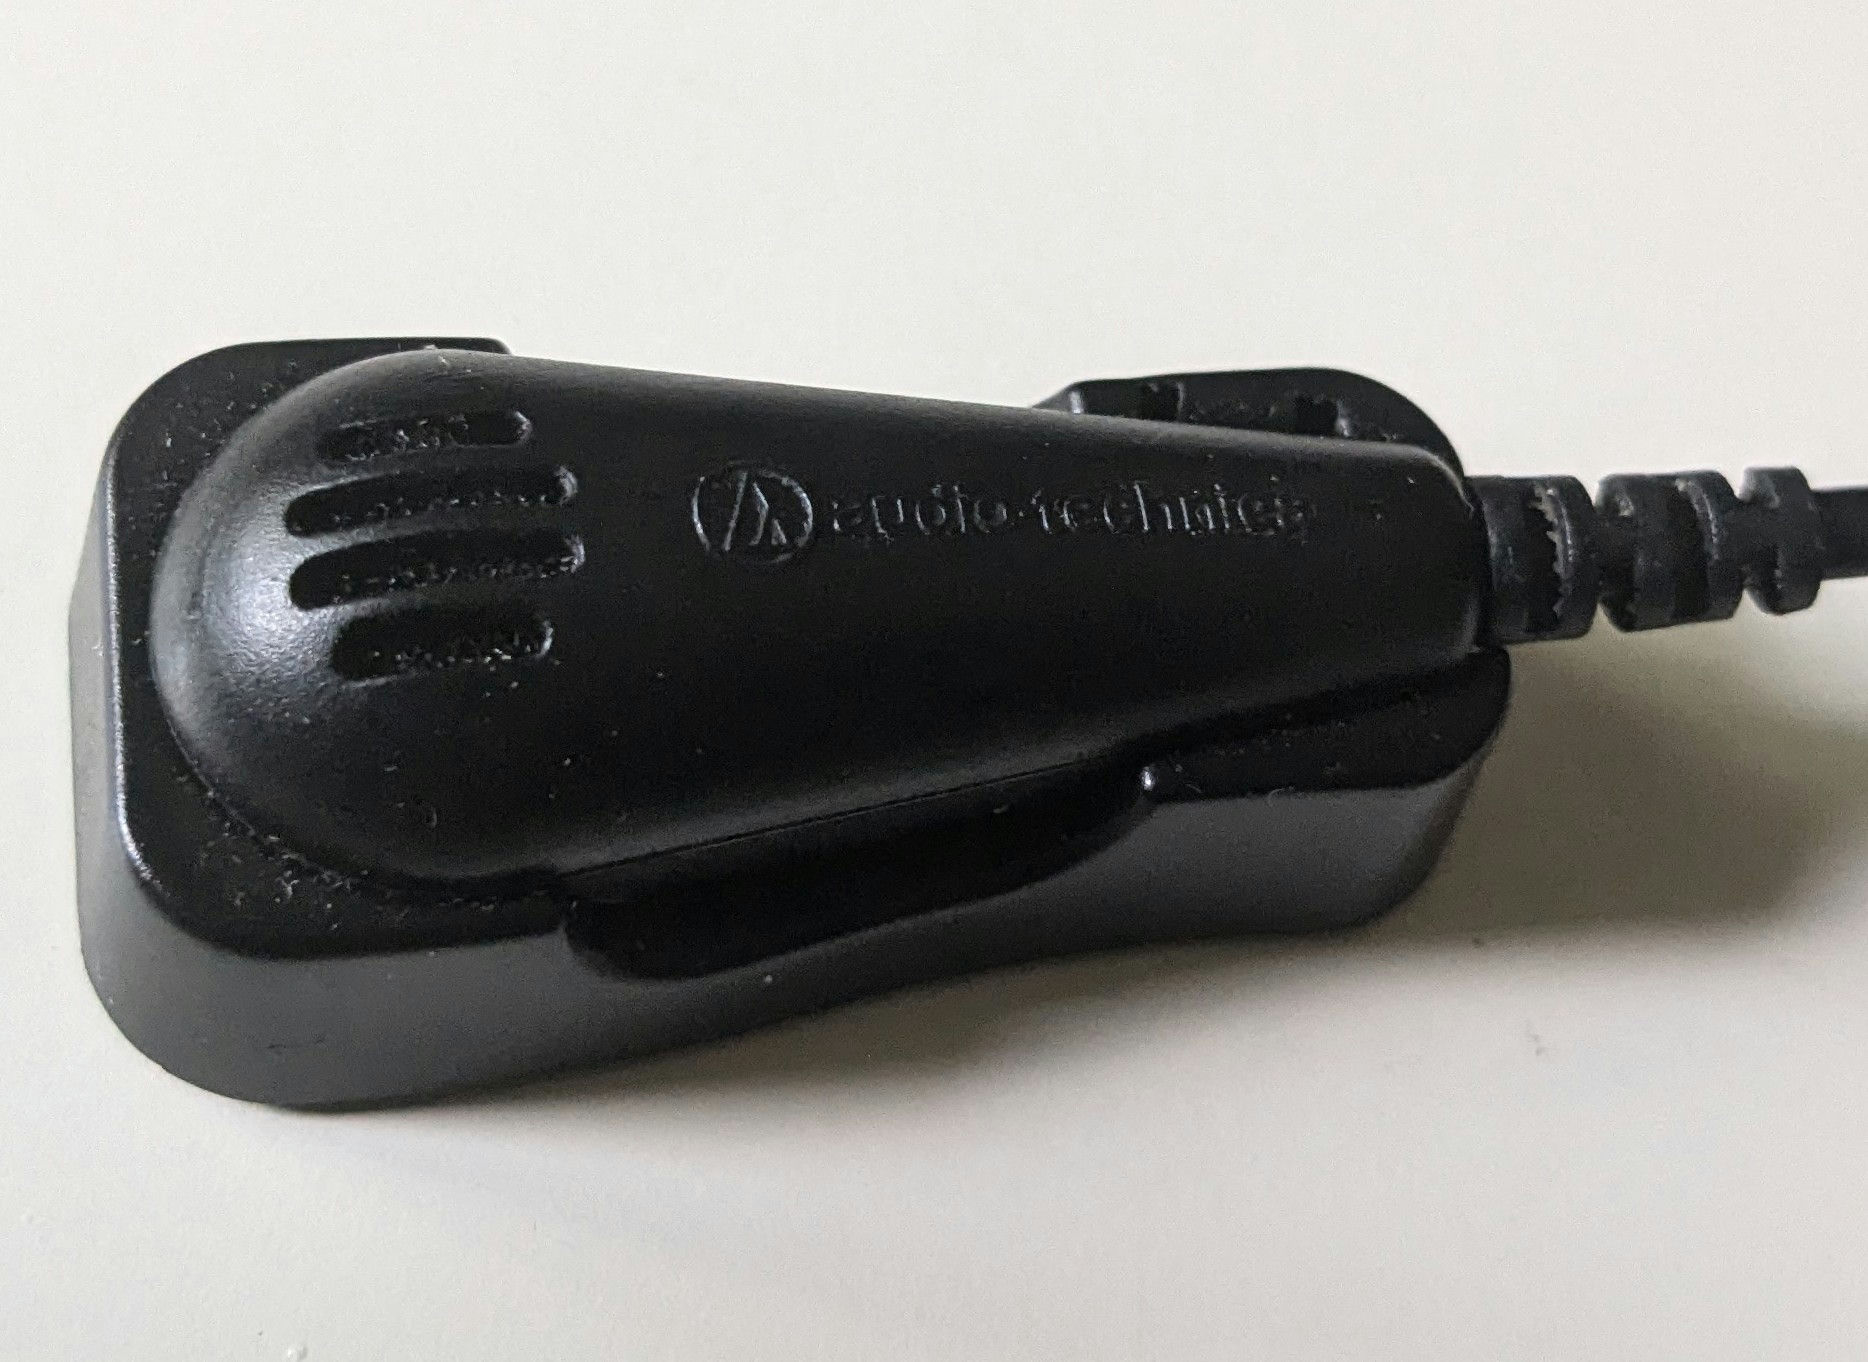
\includegraphics[width=0.35\textwidth]{images/micro_poussiereux.jpg}
\end{wrapfigure}
Lorem ipsum dolor sit amet, consectetur adipiscing elit. Integer blandit vehicula sapien ac mattis. Duis semper maximus velit vel vehicula.
Nulla quis justo sit amet sem lacinia dignissim. Donec rhoncus congue dolor in blandit. Integer nec efficitur justo. Mauris vel ex pretium,
tempus mi vel, gravida sem. Aliquam erat volutpat. Sed id finibus metus, in congue sem. Sed venenatis varius rutrum. Fusce venenatis
consectetur pulvinar. Duis tortor turpis, auctor non congue ut, suscipit eu enim. Aliquam blandit velit eu ex pulvinar, vel pharetra nisi
tincidunt. Nulla venenatis dolor sit amet est euismod, pulvinar mattis leo ornare. Nunc mattis viverra diam, sed lacinia nulla ultrices et.
Class aptent taciti sociosqu ad litora torquent per conubia nostra, per inceptos himenaeos.
Lorem ipsum dolor sit amet, consectetur adipiscing elit. Integer blandit vehicula sapien ac mattis. Duis semper maximus velit vel vehicula.
Nulla quis justo sit amet sem lacinia dignissim. Donec rhoncus congue dolor in blandit. Integer nec efficitur justo. Mauris vel ex pretium,
tempus mi vel, gravida sem. Aliquam erat volutpat. Sed id finibus metus, in congue sem. Sed venenatis varius rutrum. Fusce venenatis
consectetur pulvinar. Duis tortor turpis, auctor non congue ut, suscipit eu enim. Aliquam blandit velit eu ex pulvinar, vel pharetra nisi
tincidunt. Nulla venenatis dolor sit amet est euismod, pulvinar mattis leo ornare. Nunc mattis viverra diam, sed lacinia nulla ultrices et.
Class aptent taciti sociosqu ad litora torquent per conubia nostra, per inceptos himenaeos. 

\myparagraph{Deux images côte à côte}

\begin{figure}[h]
    \centering
    \begin{minipage}{.5\textwidth}
      \centering
      \captionsetup{width=0.9\linewidth}
      \captionof{figure}{Toujours le même micro}
      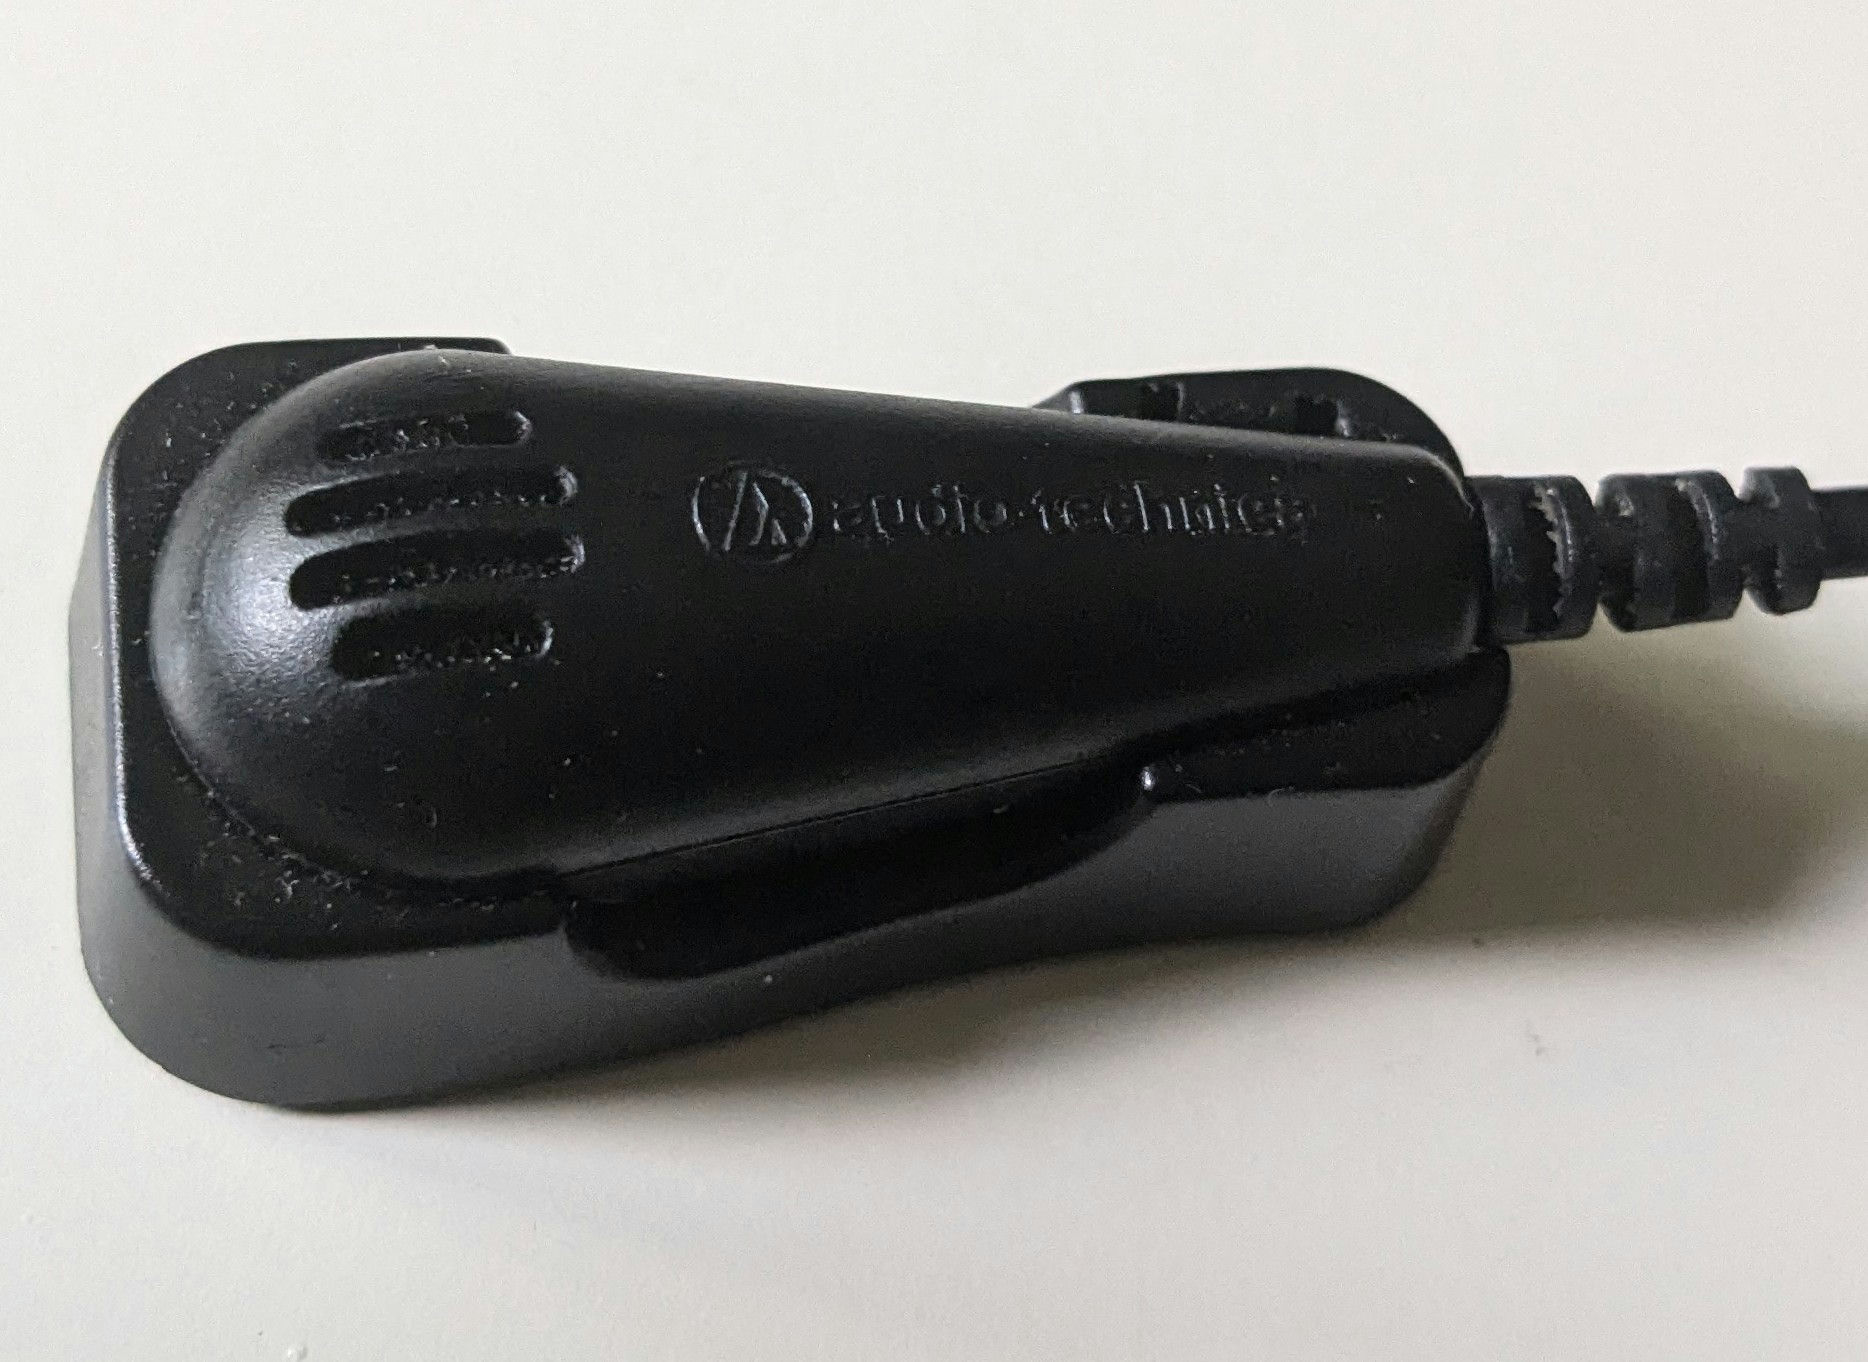
\includegraphics[width=0.9\textwidth]{images/micro_poussiereux.jpg}
    \end{minipage}%
    \begin{minipage}{.5\textwidth}
      \centering
      \captionsetup{width=0.9\linewidth}
      \captionof{figure}{Son jumeau}
      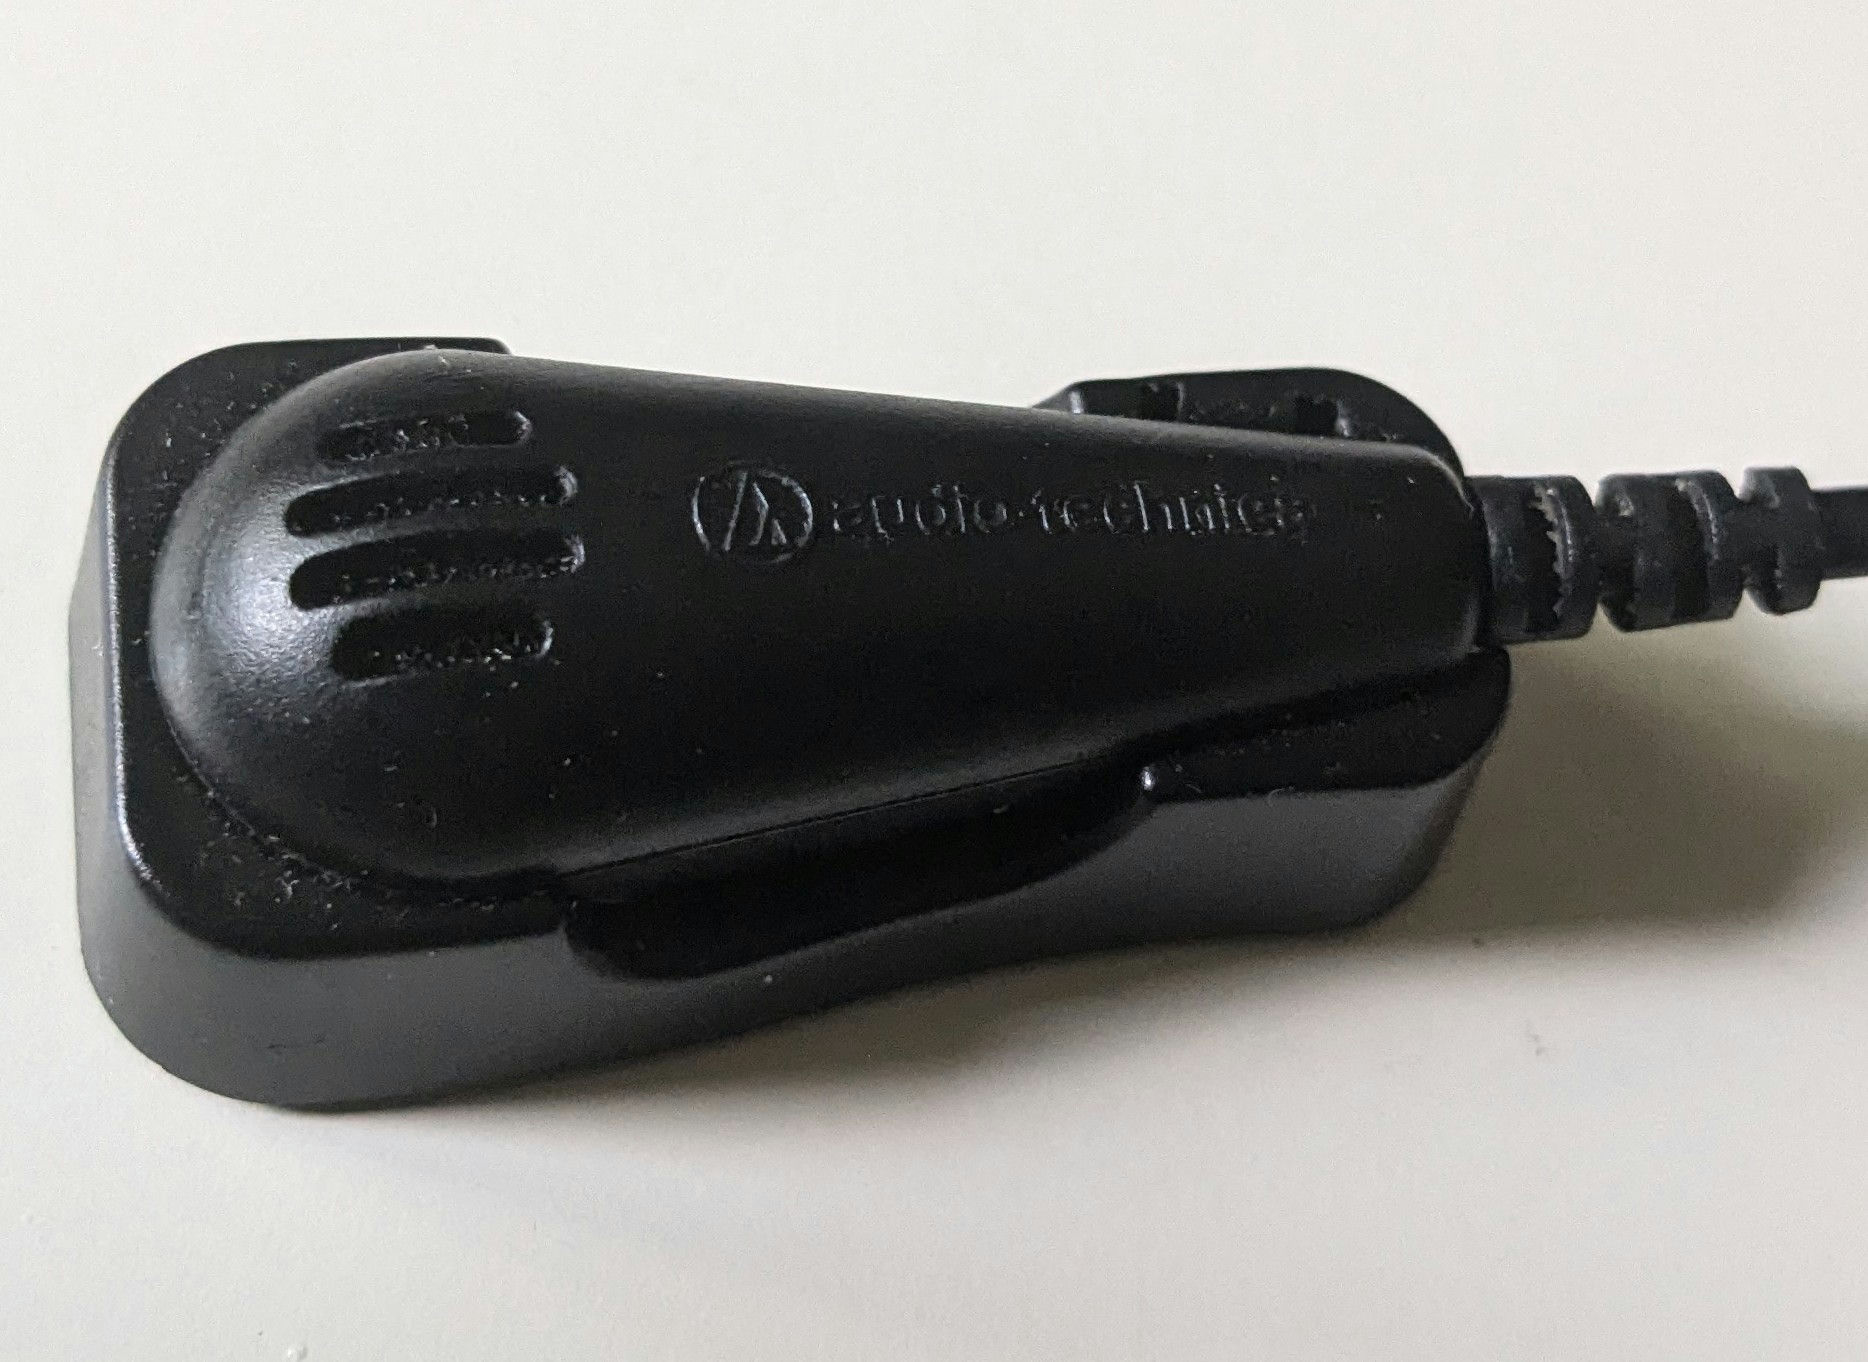
\includegraphics[width=0.9\textwidth]{images/micro_poussiereux.jpg}
    \end{minipage}
\end{figure}

\subsubsection{Tableaux}
\begin{table}[h]
    \caption[Tableau des clichés téléchargés pour 1950 – Source commune : "Remonter le temps",
    IGN]{Tableau des clichés téléchargés pour 1950 – Source commune : "Remonter le temps",
    IGN}
    \resizebox{\textwidth}{!}{%
    \begin{tabular}{|c|c|c|c|c|c|}
        \hline
        \rowcolor[RGB]{112,219,112}Identifiant de la mission & Numéro & Échelle & Type de cliché & Date de prise de vue & Nom de travail\\
        \hline
        C1224-0011\_1950\_F1024-1224\_0269 & 269 & 1/26323 & Argentique & 20/07/1950 & 11\_50\\
        \hline
        C1224-0011\_1950\_F1024-1224\_0270 & 270 & 1/26314 & Argentique & 20/07/1950 & 12\_50\\
        \hline
        C1224-0011\_1950\_F1024-1224\_0271 & 271 & 1/26315 & Argentique & 20/07/1950 & 13\_50\\
        \hline
        C1224-0011\_1950\_F1024-1224\_0272 & 272 & 1/26320 & Argentique & 20/07/1950 & 14\_50\\
        \hline
        C1224-0011\_1950\_F1024-1224\_0273 & 273 & 1/26327 & Argentique & 20/07/1950 & 15\_50\\
        \hline
        C1224-0011\_1950\_F1024-1224\_0259 & 259 & 1/26330 & Argentique & 20/07/1950 & 21\_50\\
        \hline
        C1224-0011\_1950\_F1024-1224\_0258 & 258 & 1/26323 & Argentique & 20/07/1950 & 22\_50\\
        \hline
        C1224-0011\_1950\_F1024-1224\_0257 & 257 & 1/26324 & Argentique & 20/07/1950 & 23\_50\\
        \hline
        C1224-0011\_1950\_F1024-1224\_0256 & 256 & 1/26326 & Argentique & 20/07/1950 & 24\_50\\
        \hline
        C1224-0011\_1950\_F1024-1224\_0255 & 255 & 1/26329 & Argentique & 20/07/1950 & 25\_50\\
        \hline
        C1224-0011\_1950\_F1024-1224\_0260 & 260 & 1/26334 & Argentique & 20/07/1950 & 20\_50\\
        \hline
    \end{tabular}}
\end{table} 

\subsection{Citations et biblio}

Insertion d'une citation\cite{exemple_article}